\documentclass[letterpaper,12pt]{article}

\usepackage{fullpage} % Package to use full page
\usepackage{parskip} % Package to tweak paragraph skipping
\usepackage{tikz} % Package for drawing
\usepackage{mathtools}
\usepackage{hyperref}
\usepackage{amsfonts}
\usepackage{fancyhdr}
\usepackage{times}
\usepackage{changepage}
\usepackage{amssymb}
\usepackage{amsthm}
\usepackage{amsmath}
\usepackage[spanish]{babel}
\usepackage{graphicx}
\usepackage{subcaption}
\theoremstyle{plain}
\newtheorem{theorem}{Theorem}

\usepackage{authblk} % Paquete para manejar autores y afiliaciones
\renewcommand\Authand{ y } % Cambiar "and" por "y"

\title{Trabajo práctico 1: } % Título del documento

\author[1]{Ignacio Lembo Ferrari \thanks{Correo electrónico: ignacio.lembo@ib.edu.ar}}
\affil[1]{Instituto Balseiro}
%\affil[2]{Departamento de Física, Universidad de Ejemplo}

\date{\vspace{-4ex}}

\begin{document}

\maketitle

\section{Ejercicio 1 - Mapeo de Beverton-Holt}

El mapeo de Beverton - Holt es de la forma 
\begin{equation}
    n_{t+1} = f(n_t) = \frac{r n_t}{1 + \frac{r-1}{K}n_t},
    \label{eq:beverton_holt}
\end{equation}
donde $r$ puede interpretarse como la tasa de proliferación por generación y $K$ es la capacidad de acarreo del ambiente. A pesar de ser no lineal, el modelo se puede resolver explícitamente y su solución es de la forma 
\begin{equation}
    \frac{K n_0}{n_0 + (K - n_0)r^{-t}}.
    \label{eq:beverton_sol}
\end{equation}
Debido a la forma de la solución, este mapeo puede considerarse el análogo discreto de la ecuación logística.

Los puntos de equilibrio de la ec. (\ref*{eq:beverton_holt}) satisfacen 
\begin{equation}
    n_{t+1} = n_t = \frac{r n_t}{1 + \frac{r-1}{K}n_t}.    
\end{equation}
luego resolviendo la ecuación cuadrática se llega a que $n=0$ y $n = K$ son puntos de equilibrio.

Para analizar la estabilidad de los puntos de equilibrio debemos ver para qué valores de parámetros se cumplen las siguientes condiciones 
\begin{align}
    &\left| \frac{df}{dn} \right|_{n=n^*} < 1 \Rightarrow \text{estable}, \\
    &\left| \frac{df}{dn} \right|_{n=n^*} > 1 \Rightarrow \text{inestable},
\end{align} 
luego,
\begin{equation}
    \frac{d f(n_t)}{d n_t} = \frac{r}{(1 + \frac{r-1}{K}n_t)^2} 
\end{equation}
Evaluando en los puntos de equilibrio que encontramos se tiene que 
\begin{equation}
    \left| \frac{df}{dn} \right|_{n=0} = r > 1, \hspace{1cm}
    \left| \frac{df}{dn} \right|_{n=K} = \frac{1}{r}.
\end{equation}
por lo que el punto de equilibrio $n=0$ es estable si $|r|<1$ e inestable si $|r|>1$. Por otro lado, el punto de equilibrio $n=K$ es estable si $|r|>1$ e inestable si $|r|<1$. En el caso particular en que $r=1$ se tiene que $n_{t+1} = n_t$ y el sistema es estable para cualquier valor de $K$ o $n_0$.

Graficando las ecuaciones (\ref*{eq:beverton_holt}) y (\ref*{eq:beverton_sol}) para distintos valores de $r$ y $K$ se observa que se cumplen las condiciones de estabilidad que encontramos. En la Fig. \ref*{fig:ej1_variosr_n0=1} se muestra la evolución de la población para distintos valores de $r$ y condición inicial $n_0=1$. Se observa que para $r<1$ el sistema converge a $n=0$ (extensión), para $r=1$ el sistema es estable y para $r>1$ el sistema converge a $n=K$.

\begin{figure}[h]
    \centering
    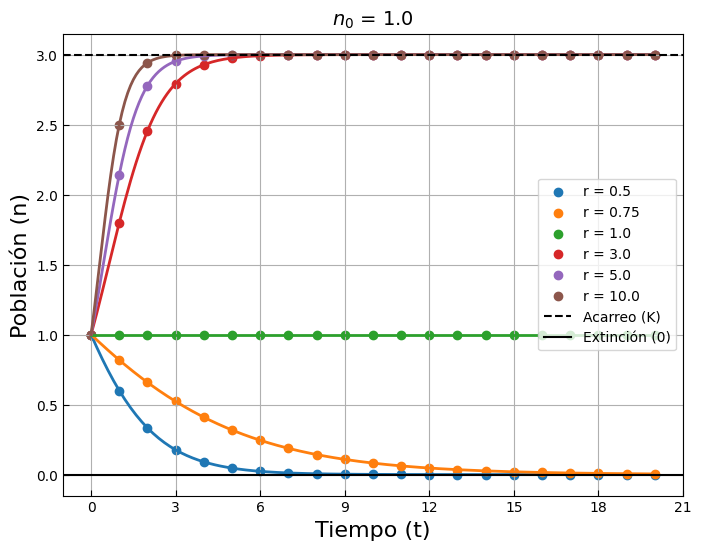
\includegraphics[width=0.7\textwidth]{ej1_variosr_n0=1.png}
    \caption{Evolución del sistema para distintos valores de $r$ y condición inicial $n_0=1$. Los puntos representan la el mapeo dado por (\ref*{eq:beverton_holt}), mientras que la linea continua representa su solución analítica (\ref*{eq:beverton_sol}).} 
    \label{fig:ej1_variosr_n0=1}
\end{figure}

En la Fig. \ref*{fig:ej1_variosn0} se muestra la evolución de la población para distintos valores de $r$ y condición inicial $n_0=5$. En \ref*{fig:ej1_variosrchico_n0=5} se observa que para $r<1$ el sistema converge a $n=0$ (extensión) y, debido a que $n_0>K$ se encuentran dos divergencias en la solución analítica ya que se anula el denominador en \ref*{eq:beverton_sol}. Por otro lado, en \ref*{fig:ej1_variosrgrande_n0=5} para $r=1$ el sistema es estable y para $r>1$ el sistema converge a $n=K$. En este último caso, no es relevante que $n_0>K$ ya que el término $(K - n_0)r^{-t}$ es siempre menor a $n_0$.

\begin{figure}[h]
    \centering
    \begin{subfigure}[b]{0.49\textwidth}
        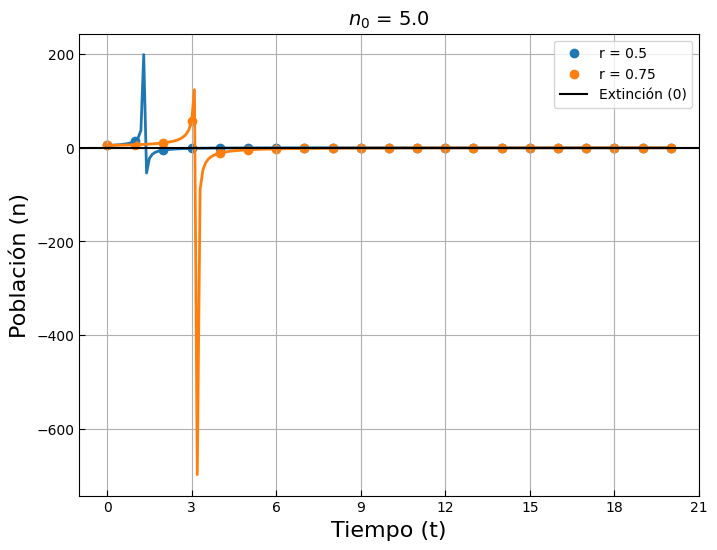
\includegraphics[width=\textwidth]{ej1_variosrchico_n0=5.png}
        \caption{}
        \label{fig:ej1_variosrchico_n0=5}
    \end{subfigure}
    \hfill
    \begin{subfigure}[b]{0.49\textwidth}
        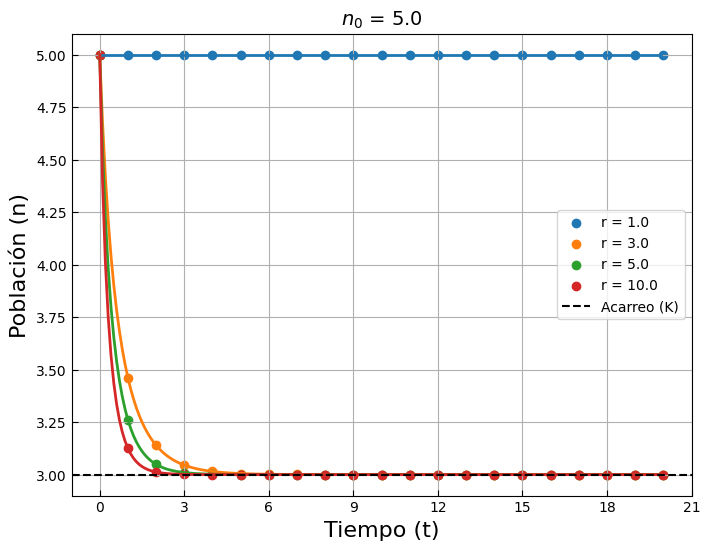
\includegraphics[width=\textwidth]{ej1_variosrgrande_n0=5.png}
        \caption{}
        \label{fig:ej1_variosrgrande_n0=5}
    \end{subfigure}
    \caption{Evolución del sistema para la condición inicial $n_0=5$. Los puntos representan la el mapeo dado por (\ref*{eq:beverton_holt}), mientras que la linea continua representa su solución analítica (\ref*{eq:beverton_sol}). (a) Valores de $r$ menores a 1 y (b) valores de $r$ mayores a 1.}
    \label{fig:ej1_variosn0}
\end{figure}


\section*{Ejercicio 2 - Ecuación logística con retraso}

Tenemos la ecuación logística con retraso
\begin{equation}
    \frac{dN}{dt} = rN(t) \biggr[ 1 - \frac{N (t - T)}{K} \biggr].
\end{equation}
Resolvemos numéricamente esta ecuación diferencial utilizando $T = 1, K = 10, r = 0.3, 1.2$ y $2.0$, $N(0) = 2$ y $T < t \leq 0$. Los resultados se encuentran en la Fig. \ref*{fig:ej2_logistica_solnumerica}. Se observa que para $r=0.3$ el sistema presenta un régimen monótono en donde la población tiende al valor de $K$. Luego, al aumentar $r=1.2$, se observan oscilaciones amortiguadas que convergen a $K$. Por último, para $r=2.0$ se observan oscilaciones sostenidas. Es decir, se observan claramente los tres regímenes.

\begin{figure}[h]
    \centering
    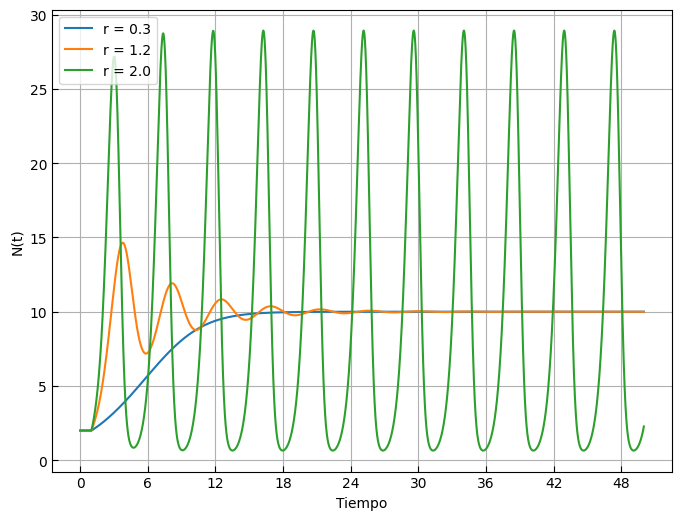
\includegraphics[width=0.7\textwidth]{ej2_logistica_solnumerica.png}
    \caption{} 
    \label{fig:ej2_logistica_solnumerica}
\end{figure}

Cuando $T$ es un poco mayor que el valor crítico $T_c = \pi/2r$, $T = T_c + \epsilon$ la ec. logística con retraso tiene la siguiente solución analítica aproximada

\begin{equation}
    N(t) \approx 1 + c e^{\frac{\epsilon t}{1 + \pi^2/4}} e^{it \biggr[ 1 - \frac{\epsilon \pi}{2 (1 + \pi^2/4)}\biggr]}.
\end{equation}

En la Fig. \ref*{fig:ej2_r=2} vemos que 

\begin{figure}[h]
    \centering
    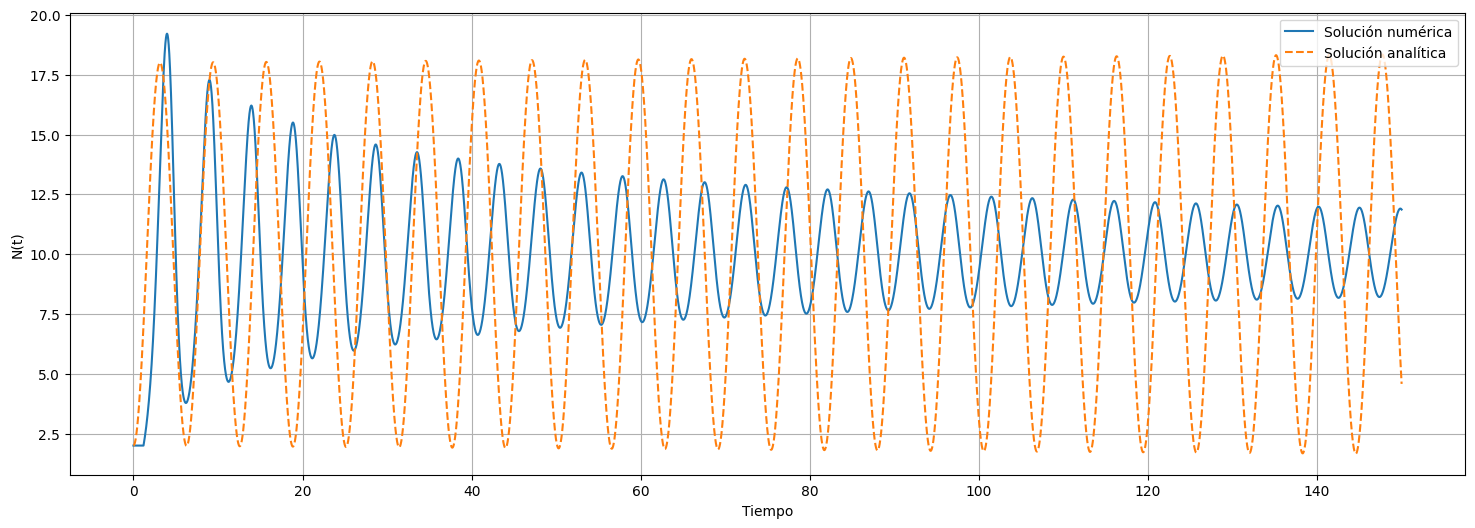
\includegraphics[width=0.7\textwidth]{ej2_r=2.png}
    \caption{} 
    \label{fig:ej2_r=2}
\end{figure}


donde $T$ es un poco mayor que el valor crítico $T_c = \pi/2r$, $T = T_c + \epsilon$. Verificar que tanto la amplitud de las oscilaciones es independiente de la condición inicial, como que su período es independiente de $r$ y aproximadamente $4T$.


\section*{Ejercicio 3 - Modelo matricial de Leslie}

En el modelo matricial de Leslie se llega a una expresión final que se interpreta como el hecho de que si una hembra deja en promedio menos de 1 descendiente en su vida, la especie se extingue, si deja 1 la especie mantiene la población y si es mayor a 1 la población crece exponencialmente. Matemáticamente corresponde a mostrar que el coeficiente asociado al crecimiento $r_1$ puede ser menor, igual o mayor a 1. Estas dos condiciones se vinculan a través de la expresión vista en clase 
$$ R = 1 - (f_0 + s_0f_1 + s_0s_1f_2 + ... + s_0s_1 ... s_{K1}). $$
Mostrar que la $r_1$ ser mayor que 1 si y solo si $R < 0$.


Sabemos que en el modelo de Leslie se llega a la siguiente expresión para los autovalores de la matriz de Leslie 
\begin{equation}
    R(r) = r^{k+1} - (f_0r^{k} + s_0f_1r^{k-1} + s_0s_1f_2r^{k-2} + ... + s_0s_1 ... s_{k-1}f_{k})
    \label{eq:polinomioLeslie}
\end{equation}
Según el teorema de Perron-Frobenius, la matriz de Leslie al ser cuadrada y no negativa invariante, dicha matriz tiene un autovector con componentes positivas, autovalor real, multiplicidad 1 y mayor en módulo que los otros autovalores. Luego, sea el autovalor $r_1$ el autovalor dominante que buscamos. 
Según el criterio de Descartes, el número de raices positivas del polinomio (ordenado de forma decreciente) es igual al número de cambios de signo de los coeficientes o menor por una diferencia par, luego vemos que en el polinomio de la ec. (\ref*{eq:polinomioLeslie}), como los coeficientes $f_i\geq0$ y $0<s_i<1$, el polinomio tiene un solo cambio de signo del primer al segundo término, por lo que se puede afirmar que el polinomio tiene una sola raiz positiva.

Ahora queremos ver que $r_1>1$ si y solo si $R<0$. Para ello, veamos que 
\begin{equation}
    R(r=0) = - f_k s_0 s_1... s_{k-1} < 0,
\end{equation}
luego, debido a que hay solo una raíz positiva y los polinomios son continuos en $r$, se tiene que $R(r)<0$ para $0<r<r_1$ y $R(r)>0$ para $r>r_1$. Por lo tanto, si $R(r=1)<0$ se tiene que $r_1>1$ y si $R(r=1)>0$ se tiene que $r_1<1$. Y vale la vuelta ya que si $r_1>1$ entonces $R(r=1)<0$ y si $r_1<1$ entonces $R(r=1)>0$.

\section{Ejercicio 4 - Especie con ciclo de vida anual}

La población de una especie con ciclo de vida anual evoluciona de acuerdo a la siguiente ecuación 
\begin{equation}
    N_{t+1} = r N_t
    \label{eq:cicloanual}
\end{equation}    
siendo $r$ la cantidad de descendientes de cada individuo. Tomando como condición inicial un solo individuo en el tiempo $t=0$, se simula el sistema para tal que $r$ obedece una distribución de Poisson con media 1.7, es decir, en cada paso de tiempo se elige un valor de $r$ de una distribución de Poisson con media 1.7. En la Fig. \ref*{fig:ej4_simulacion} se muestra la evolución del sistema para 20 pasos de tiempo. Se observa que cuando $r>1$ la población crece en el tiempo siguiente, cuando $r=1$ la población se mantiene constante y cuando $r=0$ la población se extingue. Una vez que $r=0$ la población ya se extingue para siempre, esto se puede ver directamente de la ec. (\ref*{eq:cicloanual}), ya que $N_{t+1}$ depende del valor anterior, luego si el valor anterior es nulo, esto se propagará para siempre.

\begin{figure}[h]
    \centering
    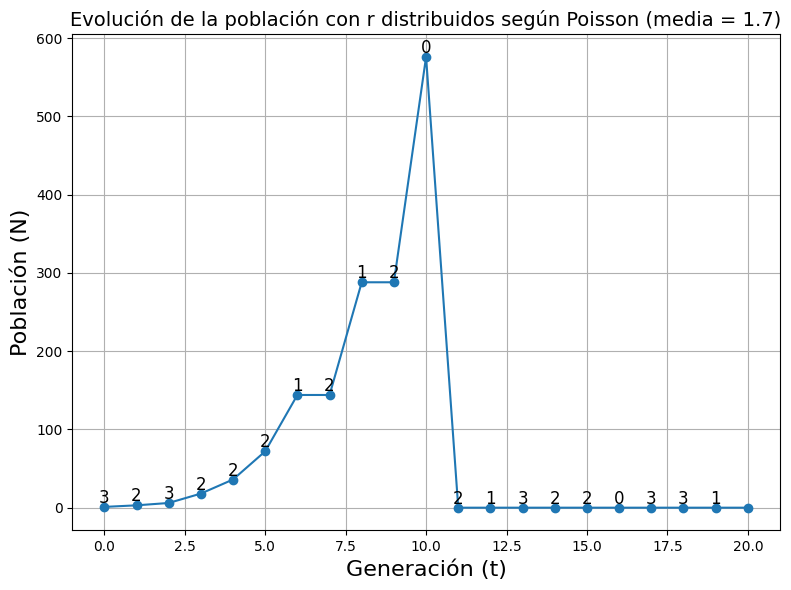
\includegraphics[width=0.7\textwidth]{ej4_simulacion.png}
    \caption{Evolución del sistema para distintos valores de $r$ y condición inicial $n_0=1$. Los puntos representan la el mapeo dado por (\ref*{eq:beverton_holt}), mientras que la linea continua representa su solución analítica (\ref*{eq:beverton_sol}).} 
    \label{fig:ej4_simulacion}
\end{figure}

Realicemos ahora $1000000$ de realizaciones del experimento anterior

Veamos la probabilidad de que la población se extinga a cada tiempo entre 1 y 20 generaciones, para ello tenemos que calcular la probabilidad de que $r$ sea distinto de 0 a tiempo t, es decir 
\begin{equation}
    P(r \ne 0) = (1 - e^{-1.7})^t.
\end{equation}

\section{Problema 5 - Animales costeros}

Para una población de animales costeros tenemos el siguiente modelo para describir su vulnerabildad ante tormentas severas, que las afectan de distinto modo según su intensidad y el estado de la marea:
\begin{itemize}
    \item Crecimiento logístico entre desastres: $ \dot{N} = f(N) = rN(1 - N/K)$.
    \item Si ocurre un desastre a tiempo $t$, inmediatamente la población se ve reducida en una fracción $p$: $N(t^+) = pN(t)$.
    \item Los tiempos entre desastres siguen una distribución exponencial con media $1/\lambda$ (es decir la ocurrencia de desastres es un proceso de Poisson, con tasa $\lambda$).
\end{itemize}
Comencemos buscando los puntos de equilibrio del crecimiento logísitco entre desastres. En este caso los puntos de equilibrio se dan cuando $\dot{N} = 0$, es decir
\begin{equation}
    f(N) = rN(1 - N/K) = 0,
\end{equation}
luego, los puntos de equilibrio son $N=0$ y $N=K$. Los estabilidad de los puntos de equilibrio está dada por el signo de la derivada de $f(N)$, es decir    
\begin{equation}
    \frac{d f(N)}{d N} = r(1 - 2N/K), 
\end{equation}
por lo tanto tomando $r>0$ se tiene que $N=0$ es inestable y $N=K$ es estable. 

La solución del crecimiento logístico es
\begin{equation}
    N(t) = \frac{K N_0 e^{rt}}{K + N_0(e^{rt} - 1)},
    \label{eq:sol_log}
\end{equation}
donde, en este problema, $N_0$ representa la población luego de una catástrofe y cuando $r>0$, $t\rightarrow\infty \Rightarrow N(t) = K$. Debemos encontrar una condición que caracterice la posibilidad del sistema de recuperarse ante un desasatre. En primer lugar, veamos que el tiempo entre desastres es $1/\lambda$. Insertando este tiempo en la solución exacta del modelo logístico (\ref*{eq:sol_log}) se tiene que 
\begin{equation}
    N(1/\lambda) = \frac{K N_0 e^{r/\lambda}}{K + N_0(e^{r/\lambda} - 1)}.
\end{equation}
Supongamos que ocurre una catastrofe, entonces un instante después de dicho evento la población será $pN_0$. Luego, la población en el siguiente intervalo de tiempo sin catástrofe seguirá la siguiente ecuación
\begin{equation}
    N(1/\lambda) = \frac{K p N_0 e^{r/\lambda}}{K + p N_0 (e^{r/\lambda} - 1)}.
\end{equation}


Cuando el sistema se encuentra cerca de la extinción ($N_0$ pequeño) podemos aproximar la solución del modelo logístico como 
\begin{equation}
    N(t) \approx p N_0 e^{r/\lambda},
\end{equation}
donde vemos que la población se recupera si $p e^{r/\lambda} > 1$ y se extingue si $p e^{r/\lambda} < 1$. Por lo tanto la condición para supervivencia de la especie es 
\begin{equation}
    p e^{r/\lambda} > 1.
\end{equation}
Verifiquemos esto con una simulación numérica. Tomamos $r=0.1, K=100, p=0.1, \lambda=0.1$ y $N_0=1$. En la Fig. \ref*{fig:ej5} se muestra la evolución del sistema para 20 pasos de tiempo. Se observa que la población se recupera si $p e^{r/\lambda} > 1$ y se extingue si $p e^{r/\lambda} < 1$.

\begin{figure}[h]
    \centering
    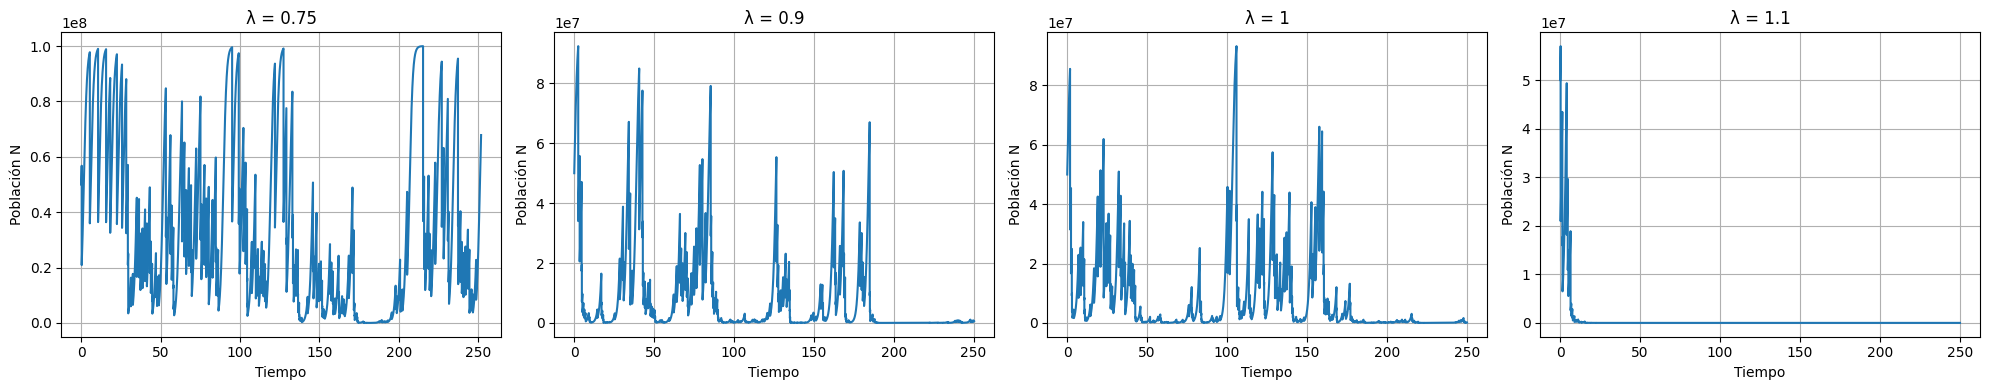
\includegraphics[width=0.7\textwidth]{ej5.png}
    \caption{} 
    \label{fig:ej5}
\end{figure}



\section{Ejercicio 6 - Efecto Allee}



El efecto Allee da cuenta de un fenómeno, descripto por W.C. Allee, asociado a la existencia de un número crítico mínimo de individuos para garantizar la supervivencia de la especie. Se supone que a partir de cierto umbral, el tamaño poblacional es tan reducido que los individuos no se reproducen al no encontrarse con otros individuos de la misma población. Una manera de modelar este efecto es por medio de la siguiente ecuación. 
\begin{equation}
    \frac{dN}{dt} = rN \biggr[ 1 - \frac{N}{K} \biggr] \biggr[ \frac{N}{A} -1 \biggr]. 
\end{equation}

Analizar sus equilibrios y la estabilidad de los mismos. ¿Qué la hace diferente de la logística?










%\bibliographystyle{plain} % Estilo de bibliografía
%\bibliography{bibliography}    % Nombre de tu archivo .bib sin la extensión

\end{document}